%-----------------------------------------------------------------------------------------------------------------------------------------------%
%	The MIT License (MIT)
%
%	Copyright (c) 2021 Philip Empl
%
%	Permission is hereby granted, free of charge, to any person obtaining a copy
%	of this software and associated documentation files (the "Software"), to deal
%	in the Software without restriction, including without limitation the rights
%	to use, copy, modify, merge, publish, distribute, sublicense, and/or sell
%	copies of the Software, and to permit persons to whom the Software is
%	furnished to do so, subject to the following conditions:
%	
%	THE SOFTWARE IS PROVIDED "AS IS", WITHOUT WARRANTY OF ANY KIND, EXPRESS OR
%	IMPLIED, INCLUDING BUT NOT LIMITED TO THE WARRANTIES OF MERCHANTABILITY,
%	FITNESS FOR A PARTICULAR PURPOSE AND NONINFRINGEMENT. IN NO EVENT SHALL THE
%	AUTHORS OR COPYRIGHT HOLDERS BE LIABLE FOR ANY CLAIM, DAMAGES OR OTHER
%	LIABILITY, WHETHER IN AN ACTION OF CONTRACT, TORT OR OTHERWISE, ARISING FROM,
%	OUT OF OR IN CONNECTION WITH THE SOFTWARE OR THE USE OR OTHER DEALINGS IN
%	THE SOFTWARE.
%	
%
%-----------------------------------------------------------------------------------------------------------------------------------------------%


%============================================================================%
%
%	DOCUMENT DEFINITION
%
%============================================================================%

\documentclass[10pt,A4,english]{article}	


%----------------------------------------------------------------------------------------
%	ENCODING
%----------------------------------------------------------------------------------------

% we use utf8 since we want to build from any machine
\usepackage[utf8]{inputenc}		
\usepackage[USenglish]{isodate}
\usepackage{fancyhdr}
\usepackage[numbers]{natbib}

%----------------------------------------------------------------------------------------
%	LOGIC
%----------------------------------------------------------------------------------------

% provides \isempty test
\usepackage{xstring, xifthen}
\usepackage{enumitem}
\usepackage[english]{babel}
\usepackage{blindtext}
\usepackage{pdfpages}
\usepackage{changepage}
%----------------------------------------------------------------------------------------
%	FONT BASICS
%----------------------------------------------------------------------------------------

% some tex-live fonts - choose your own

%\usepackage[defaultsans]{droidsans}
%\usepackage[default]{comfortaa}
%\usepackage{cmbright}
\usepackage[default]{raleway}
%\usepackage{fetamont}
%\usepackage[default]{gillius}
%\usepackage[light,math]{iwona}
%\usepackage[thin]{roboto} 

% set font default
% \renewcommand*\familydefault{\sfdefault} 	
% \usepackage[T1]{fontenc}
\usepackage{newtxtext,newtxmath}

% more font size definitions
\usepackage{moresize}

%----------------------------------------------------------------------------------------
%	FONT AWESOME ICONS
%---------------------------------------------------------------------------------------- 

% include the fontawesome icon set
\usepackage{fontawesome}

% use to vertically center content
% credits to: http://tex.stackexchange.com/questions/7219/how-to-vertically-center-two-images-next-to-each-other
\newcommand{\vcenteredinclude}[1]{\begingroup
\setbox0=\hbox{\includegraphics{#1}}%
\parbox{\wd0}{\box0}\endgroup}
\newcommand{\tab}[1]{\hspace{.2\textwidth}\rlap{#1}}
% use to vertically center content
% credits to: http://tex.stackexchange.com/questions/7219/how-to-vertically-center-two-images-next-to-each-other
\newcommand*{\vcenteredhbox}[1]{\begingroup
\setbox0=\hbox{#1}\parbox{\wd0}{\box0}\endgroup}

% icon shortcut
\newcommand{\icon}[3] { 							
	\makebox(#2, #2){\textcolor{maincol}{\csname fa#1\endcsname}}
}	


% icon with text shortcut
\newcommand{\icontext}[4]{ 						
	\vcenteredhbox{\icon{#1}{#2}{#3}}  \hspace{2pt}  \parbox{0.9\mpwidth}{\textcolor{#4}{#3}}
}

% icon with website url
\newcommand{\iconhref}[5]{ 						
    \vcenteredhbox{\icon{#1}{#2}{#5}}  \hspace{2pt} \href{#4}{\textcolor{#5}{#3}}
}

% icon with email link
\newcommand{\iconemail}[5]{ 						
    \vcenteredhbox{\icon{#1}{#2}{#5}}  \hspace{2pt} \href{mailto:#4}{\textcolor{#5}{#3}}
}

%----------------------------------------------------------------------------------------
%	PAGE LAYOUT  DEFINITIONS
%----------------------------------------------------------------------------------------

% page outer frames (debug-only)
% \usepackage{showframe}		

% we use paracol to display breakable two columns
\usepackage{paracol}
\usepackage{tikzpagenodes}
\usetikzlibrary{calc}
\usepackage{lmodern}
\usepackage{multicol}
\usepackage{lipsum}
\usepackage{atbegshi}
% define page styles using geometry
\usepackage[a4paper]{geometry}

% remove all possible margins
\geometry{top=1cm, bottom=1cm, left=1cm, right=1cm}

\usepackage{fancyhdr}
\pagestyle{empty}

% space between header and content
% \setlength{\headheight}{0pt}

% indentation is zero
\setlength{\parindent}{0mm}

%----------------------------------------------------------------------------------------
%	TABLE /ARRAY DEFINITIONS
%---------------------------------------------------------------------------------------- 

% extended aligning of tabular cells
\usepackage{array}

% custom column right-align with fixed width
% use like p{size} but via x{size}
\newcolumntype{x}[1]{%
>{\raggedleft\hspace{0pt}}p{#1}}%


%----------------------------------------------------------------------------------------
%	GRAPHICS DEFINITIONS
%---------------------------------------------------------------------------------------- 

%for header image
\usepackage{graphicx}

% use this for floating figures
% \usepackage{wrapfig}
% \usepackage{float}
% \floatstyle{boxed} 
% \restylefloat{figure}

%for drawing graphics		
\usepackage{tikz}			
\usepackage{ragged2e}	
\usetikzlibrary{shapes, backgrounds,mindmap, trees}

%----------------------------------------------------------------------------------------
%	Color DEFINITIONS
%---------------------------------------------------------------------------------------- 
\usepackage{transparent}
\usepackage{color}

% primary color
\definecolor{maincol}{RGB}{ 64,64,64}

% accent color, secondary
% \definecolor{accentcol}{RGB}{ 250, 150, 10 }

% dark color
\definecolor{darkcol}{RGB}{ 70, 70, 70 }

% light color
\definecolor{lightcol}{RGB}{245,245,245}

% \definecolor{accentcol}{RGB}{59,77,97}
\definecolor{accentcol}{RGB}{75,118,166}



% Package for links, must be the last package used
\usepackage[hidelinks]{hyperref}

% returns minipage width minus two times \fboxsep
% to keep padding included in width calculations
% can also be used for other boxes / environments
\newcommand{\mpwidth}{\linewidth-\fboxsep-\fboxsep}
	


%============================================================================%
%
%	CV COMMANDS
%
%============================================================================%

%----------------------------------------------------------------------------------------
%	 CV LIST
%----------------------------------------------------------------------------------------

% renders a standard latex list but abstracts away the environment definition (begin/end)
\newcommand{\cvlist}[1] {
	\begin{itemize}{#1}\end{itemize}
}

%----------------------------------------------------------------------------------------
%	 CV TEXT
%----------------------------------------------------------------------------------------

% base class to wrap any text based stuff here. Renders like a paragraph.
% Allows complex commands to be passed, too.
% param 1: *any
\newcommand{\cvtext}[1] {
	\begin{tabular*}{1\mpwidth}{p{0.98\mpwidth}}
		\parbox{1\mpwidth}{#1}
	\end{tabular*}
}
\newcommand{\cvtextsmall}[1] {
	\begin{tabular*}{0.8\mpwidth}{p{0.8\mpwidth}}
		\parbox{0.8\mpwidth}{#1}
	\end{tabular*}
}
%----------------------------------------------------------------------------------------
%	CV SECTION
%----------------------------------------------------------------------------------------

% Renders a a CV section headline with a nice underline in main color.
% param 1: section title
\newcommand{\cvsection}[1] {
	\vspace{14pt}
	\cvtext{
		\textbf{\LARGE{\textcolor{darkcol}{#1}}}\\[-4pt]
		\textcolor{accentcol}{ \rule{0.2\textwidth}{1.5pt} } \\
	}
}

\newcommand{\cvsectionsmall}[1] {
	\vspace{14pt}
	\cvtext{
		\textbf{\Large{\textcolor{darkcol}{#1}}}\\[-4pt]
		\textcolor{accentcol}{ \rule{0.2\textwidth}{1.5pt} } \\
	}
}

\newcommand{\cvheadline}[1] {
	\vspace{16pt}
	\cvtext{
		\textbf{\Huge{\textcolor{accentcol}{#1}}}\\[-4pt]
		 
	}
}

\newcommand{\cvsubheadline}[1] {
	\vspace{16pt}
	\cvtext{
		\textbf{\huge{\textcolor{darkcol}{#1}}}\\[-4pt]
		 
	}
}
%----------------------------------------------------------------------------------------
%	META SKILL
%----------------------------------------------------------------------------------------

% Renders a progress-bar to indicate a certain skill in percent.
% param 1: name of the skill / tech / etc.
% param 2: level (for example in years)
% param 3: percent, values range from 0 to 1
\newcommand{\cvskill}[3] {
	\begin{tabular*}{1\mpwidth}{p{0.72\mpwidth}  r}
 		\textcolor{black}{\textbf{#1}} & \textcolor{maincol}{#2}\\
	\end{tabular*}%
	
	\hspace{4pt}
	\begin{tikzpicture}[scale=1,rounded corners=2pt,very thin]
		\fill [lightcol] (0,0) rectangle (1\mpwidth, 0.15);
		\fill [accentcol] (0,0) rectangle (#3\mpwidth, 0.15);
  	\end{tikzpicture}%
}


%----------------------------------------------------------------------------------------
%	 CV EVENT
%----------------------------------------------------------------------------------------

% Renders a table and a paragraph (cvtext) wrapped in a parbox (to ensure minimum content
% is glued together when a pagebreak appears).
% Additional Information can be passed in text or list form (or other environments).
% the work you did
% param 1: time-frame i.e. Sep 14 - Jan 15 etc.
% param 2:	 event name (job position etc.)
% param 3: Customer, Employer, Industry
% param 4: Short description
% param 5: work done (optional)
% param 6: technologies include (optional)
% param 7: achievements (optional)
\newcommand{\cvevent}[7] {
	
	% we wrap this part in a parbox, so title and description are not separated on a pagebreak
	% if you need more control on page breaks, remove the parbox
	\parbox{\mpwidth}{
		\begin{tabular*}{1\mpwidth}{p{0.66\mpwidth}  r}
	 		\textcolor{black}{\textbf{#2}} & \colorbox{accentcol}{\makebox[0.32\mpwidth]{\textcolor{white}{\textbf{#1}}}} \\
			\textcolor{maincol}{#3} & \\
		\end{tabular*}\\[8pt]
	
		\ifthenelse{\isempty{#4}}{}{
			\cvtext{#4}\\
		}
	}
	\vspace{14pt}
}


%----------------------------------------------------------------------------------------
%	 CV META EVENT
%----------------------------------------------------------------------------------------

% Renders a CV event on the sidebar
% param 1: title
% param 2: subtitle (optional)
% param 3: customer, employer, etc,. (optional)
% param 4: info text (optional)
\newcommand{\cvmetaevent}[4] {
	\textcolor{maincol} { \cvtext{\textbf{\begin{flushleft}#1\end{flushleft}}}}

	\ifthenelse{\isempty{#2}}{}{
	\textcolor{black} {\cvtext{\textbf{#2}} }
	}

	\ifthenelse{\isempty{#3}}{}{
		\cvtext{{ \textcolor{maincol} {#3} }}\\
	}

	\cvtext{#4}\\[14pt]
}

%---------------------------------------------------------------------------------------
%	QR CODE
%----------------------------------------------------------------------------------------

% Renders a qrcode image (centered, relative to the parentwidth)
% param 1: percent width, from 0 to 1
\newcommand{\cvqrcode}[1] {
	\begin{center}
		\includegraphics[width={#1}\mpwidth]{qrcode}
	\end{center}
}


% HEADER AND FOOOTER 
%====================================
\newcommand\Header[1]{%
\begin{tikzpicture}[remember picture,overlay]
\fill[accentcol]
  (current page.north west) -- (current page.north east) --
  ([yshift=50pt]current page.north east|-current page text area.north east) --
  ([yshift=50pt,xshift=-3cm]current page.north|-current page text area.north) --
  ([yshift=10pt,xshift=-5cm]current page.north|-current page text area.north) --
  ([yshift=10pt]current page.north west|-current page text area.north west) -- cycle;
\node[font=\sffamily\bfseries\color{white},anchor=west,
  xshift=0.7cm,yshift=-0.32cm] at (current page.north west)
  {\fontsize{12}{12}\selectfont {#1}};
\end{tikzpicture}%
}

\usepackage{lastpage}
\usepackage{fancyhdr}

% \newcommand\Footer[1]{%
% \begin{tikzpicture}[remember picture,overlay]
% \fill[lightcol]
%   (current page.south east) -- (current page.south west) --
%   ([yshift=-80pt]current page.south east|-current page text area.south east) --
%   ([yshift=-80pt,xshift=-6cm]current page.south|-current page text area.south) --
%   ([xshift=-2.5cm,yshift=-10pt]current page.south|-current page text area.south) --	
%   ([yshift=-10pt]current page.south east|-current page text area.south east) -- cycle;
% \node[yshift=0.32cm,xshift=9cm] at (current page.south) {\fontsize{10}{10}\selectfont \textbf{\thepage}};
% \end{tikzpicture}%
% }

\newcommand\Footer[1]{%
\begin{tikzpicture}[remember picture,overlay]
\fill[lightcol]
  (current page.south east) -- (current page.south west) --
  ([yshift=-80pt]current page.south east|-current page text area.south east) --
  ([yshift=-80pt,xshift=-6cm]current page.south|-current page text area.south) --
  ([xshift=-2.5cm,yshift=-10pt]current page.south|-current page text area.south) --  
  ([yshift=-10pt]current page.south east|-current page text area.south east) -- cycle;
\node[yshift=0.32cm,xshift=9cm] at (current page.south) {\fontsize{10}{10}\selectfont {\thepage} of \pageref{LastPage}};
\node[yshift=0.4cm,xshift=1.8cm] at (current page.south) {\fontsize{7}{7}\selectfont I hereby consent to my personal data being processed for the purpose of considering};
\node[yshift=0.14cm,xshift=-0.2cm] at (current page.south) {\fontsize{7}{7}\selectfont my application for the vacancy advertised.};
\end{tikzpicture}%
}


%=====================================
%============================================================================%
%
%
%
%	DOCUMENT CONTENT
%
%
%
%============================================================================%
\begin{document}

\columnratio{0.31}
\setlength{\columnsep}{2.2em}
\setlength{\columnseprule}{4pt}
\colseprulecolor{white}


% LEBENSLAUF HIERE
\AtBeginShipoutFirst{\Header{CV}\Footer{1}}
\AtBeginShipout{\AtBeginShipoutAddToBox{\Header{CV - Paweł Bujakiewicz}\Footer{2}}}

\newpage

\colseprulecolor{lightcol}
\columnratio{0.31}
\setlength{\columnsep}{2.2em}
\setlength{\columnseprule}{4pt}
\begin{paracol}{2}


\begin{leftcolumn}
%---------------------------------------------------------------------------------------
%	META IMAGE
%----------------------------------------------------------------------------------------
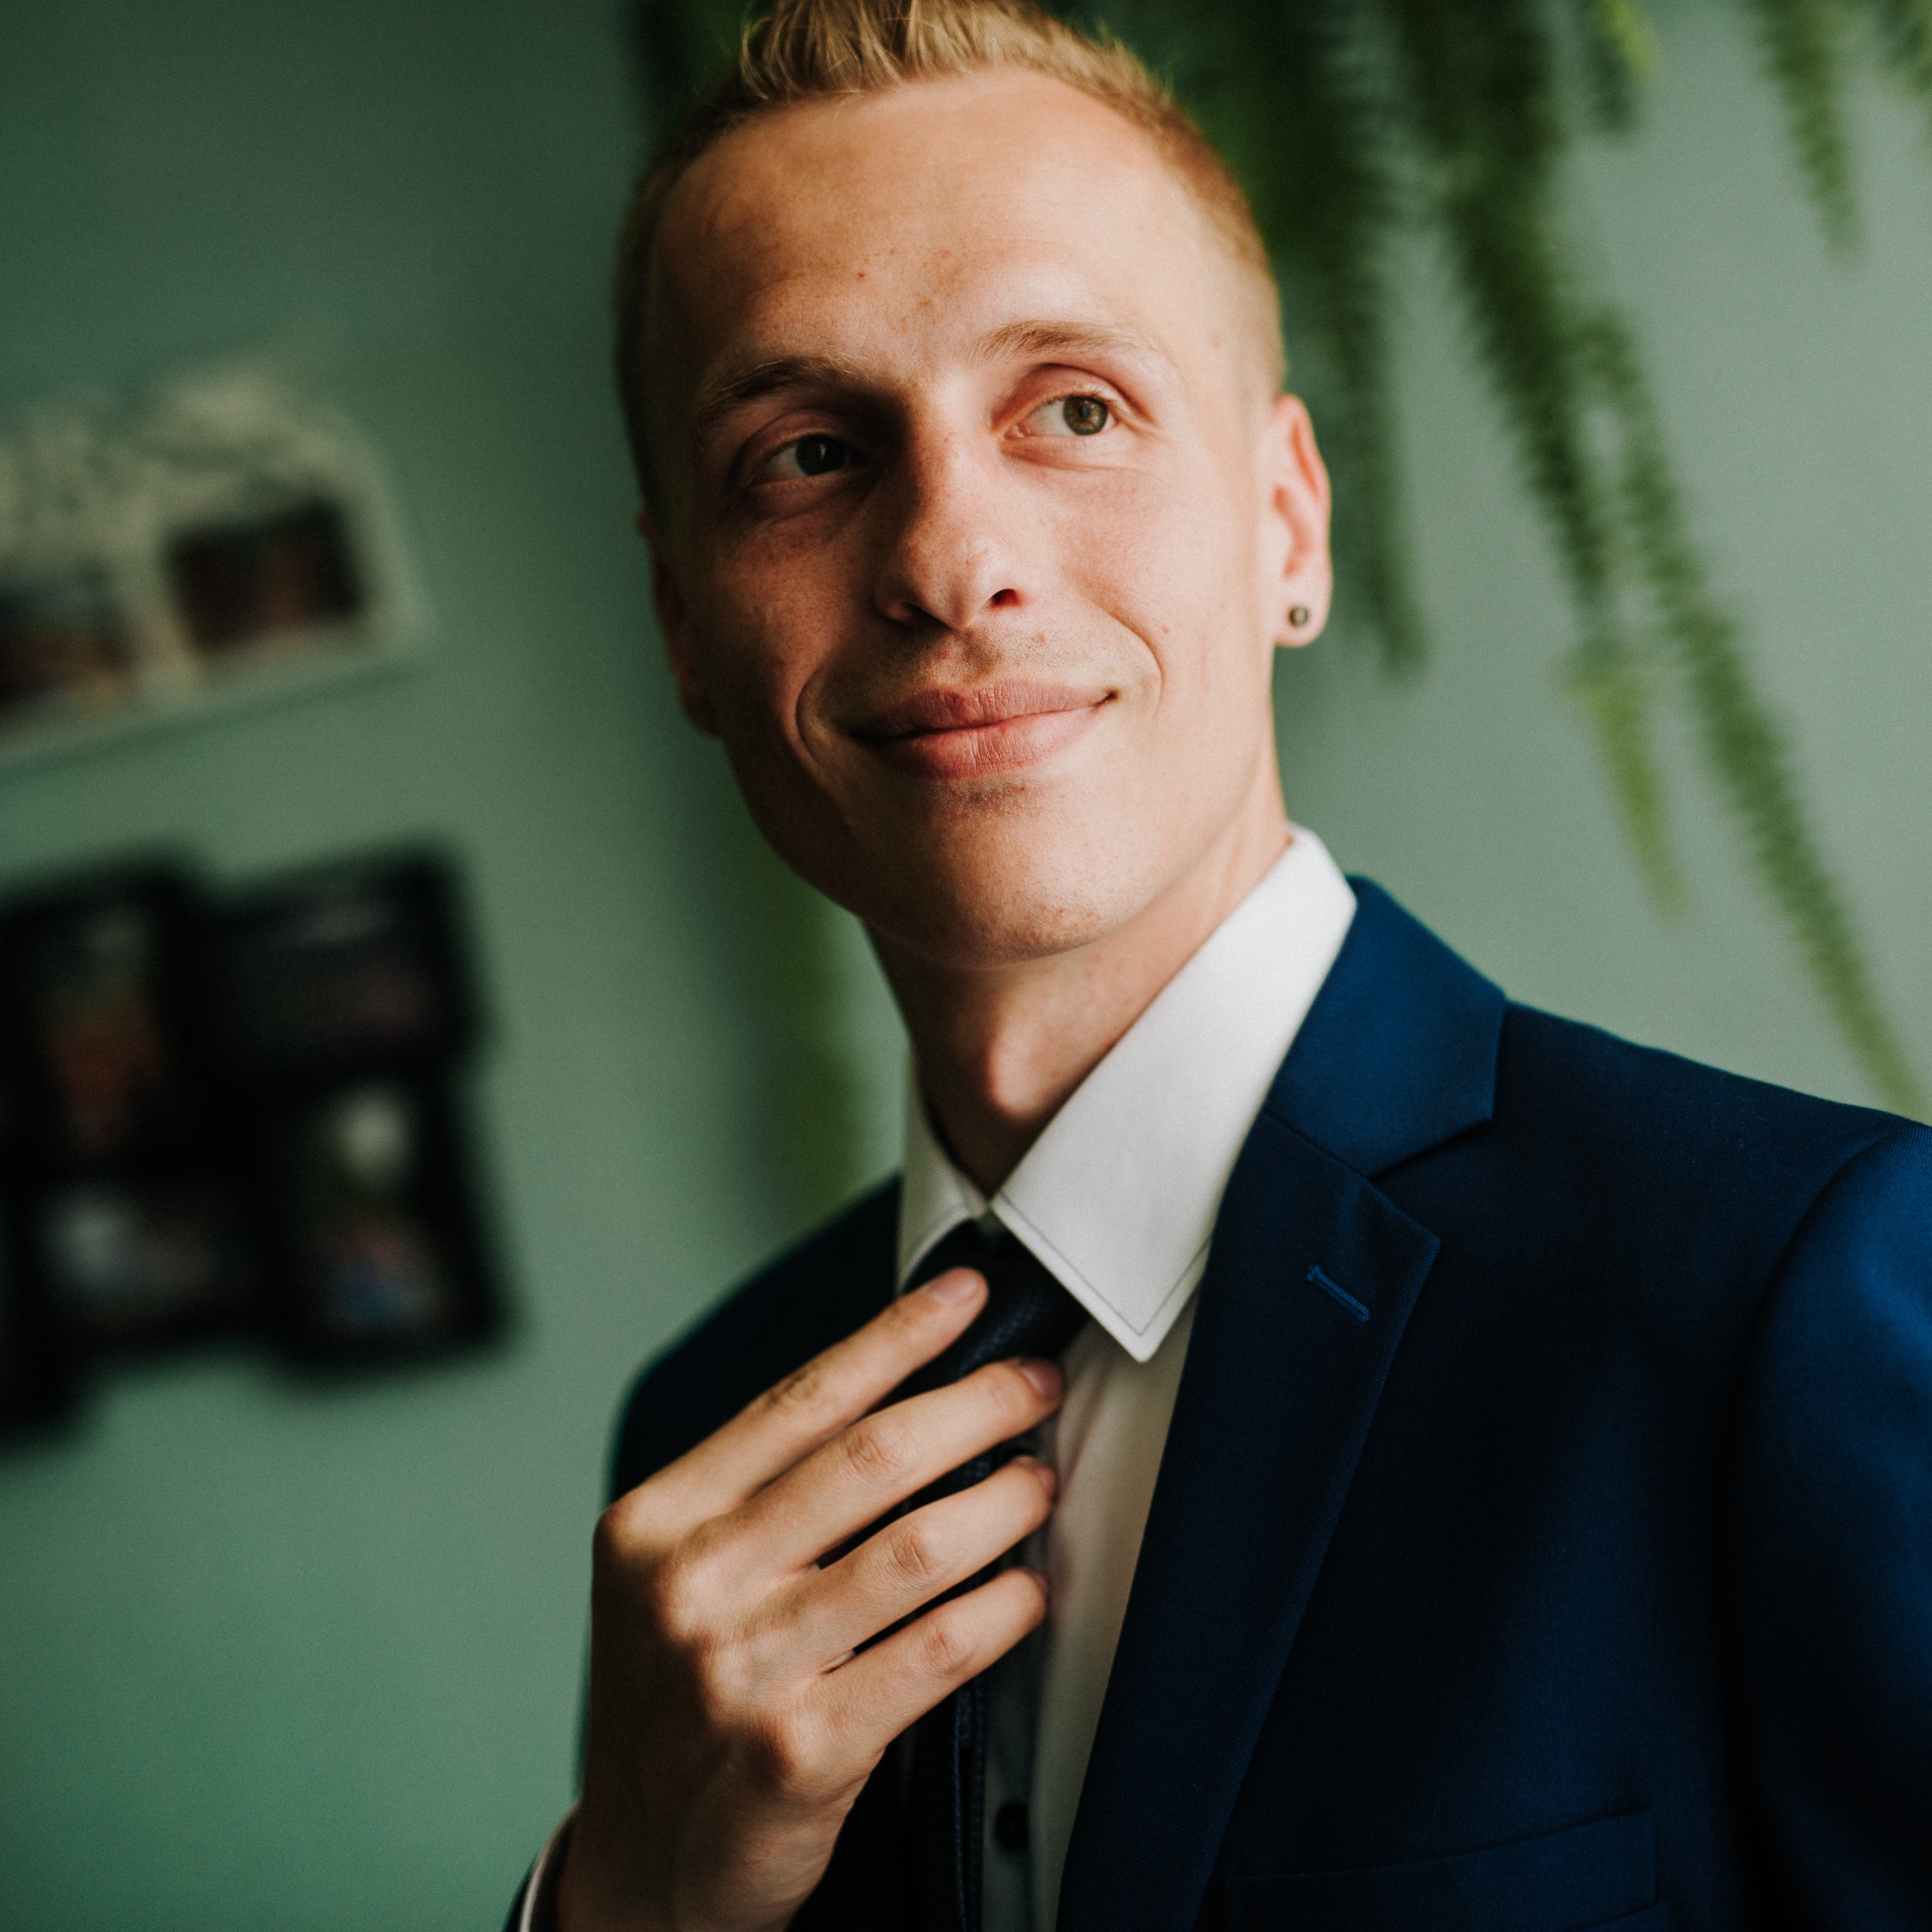
\includegraphics[width=\linewidth]{BujakiewiczPawel.jpg}	%trimming relative to image size

%---------------------------------------------------------------------------------------
%	META SKILLS
%----------------------------------------------------------------------------------------
	\fcolorbox{white}{white}{\begin{minipage}[c][1.5cm][c]{1\mpwidth}
		\LARGE{\textbf{\textcolor{accentcol}{Paweł Bujakiewicz}}} \\[2pt]
		\normalsize{ \textcolor{maincol} {Devops Engineer} }
\end{minipage}} \\
\icontext{BirthdayCake}{12}{Date of birth: 06/29/1989}{black}\\[6pt]
\icontext{MapMarker}{12}{Address: Gdańsk}{black}\\[6pt]



\cvsection{Skills}

\cvskill{OKD \newline OpenShift} {4+ yrs.} {0.9} \\[-2pt]

\cvskill{Kubernetes} {4+ yrs.} {0.7} \\[-2pt]

\cvskill{GCP} {3+ yrs.} {0.6} \\[-2pt]

\cvskill{Azure} {0+ yrs.} {0.2} \\[-2pt]

\cvskill{Docker} {5+ yrs.} {0.8} \\[-2pt]

\cvskill{Linux} {10+ yrs.} {0.9} \\[-2pt]

\cvskill{CI/CD \newline GitOps} {5+ yrs.} {0.8} \\[-2pt]

\cvskill{Chef \newline Ansible} {4+ yrs.} {0.7} \\[-2pt]

\cvskill{Terraform} {2+ yrs.} {0.5} \\[-2pt]

\cvskill{GrayLog} {4+ yrs.} {0.7} \\[-2pt]

\cvskill{Prometheus} {4+ yrs.} {0.8} \\[-2pt]

\cvskill{Bash} {10+ yrs.} {0.8} \\[-2pt]

\cvskill{Jira \newline Confluence} {4+ yrs.} {0.6} \\[-2pt]


\newpage


%---------------------------------------------------------------------------------------
%	SOFT SKILLS
%----------------------------------------------------------------------------------------
\cvsection{Soft Skills}

\icontext{CaretRight}{12}{Can't stop learning}{black}\\[6pt]
\icontext{CaretRight}{12}{Teamwork}{black}\\[6pt]
\icontext{CaretRight}{12}{Independent}{black}\\[6pt]
\icontext{CaretRight}{12}{Knowledge-sharing}{black}\\[6pt]

%---------------------------------------------------------------------------------------
%	LANGUAGES
%----------------------------------------------------------------------------------------
\cvsection{Languages}

\icontext{CaretRight}{12}{Polish: Native}{black}\\[6pt]
\icontext{CaretRight}{12}{English: B1 - Intermediate}{black}\\[6pt]

%---------------------------------------------------------------------------------------
%	EDUCATION
%----------------------------------------------------------------------------------------
\cvsection{Education}

\cvmetaevent
{10/2010 - 02/2014}
{Electronics and Computer Science}
{Koszalin University of Technology}
{\textit{Computer Science • full-time} \newline Engineering thesis: \glqq Management of rights in the local network based on the RBAC (Role-Based Access Control) method.\grqq.}

\cvmetaevent
{09/2005 - 06/2010}
{IT technical school}
{AGRICULTURAL SCHOOL GROUP, Practical Training Center name of Stefana Żeromskiego in Świdwin}
{\textit{Computer technician}}


%
%\cvsection{Projekte}

%	\cvlist{
%		\item \hyperlink{https://github.com/philipempl/ether-twin}{\textbf{Ether-Twin.}}\\ Ethereum Applikation für Digital Twins.
%		\item \hyperlink{https://github.com/philipempl/Peter-Pan}{\textbf{Peter Pan.}}\\ Koch-App (t.b.a.).
%		\item \hyperlink{https://github.com/philipempl/Innovation-Tool}{\textbf{Innovation Tool.}}\\ Webcrawler für \hyperlink{https://ibi.de/}{Ibi}.
%		\item \hyperlink{https://github.com/philipempl/cozone}{\textbf{COZONE.}} \\ Soziales Netzwerk (t.b.a.).
%		\item \hyperlink{https://github.com/geritwagner/enlit}{\textbf{ENLIT.}}\\ Exploring new Literature (Bachelorarbeit).
%		\item \textbf{Crowdfunding.} \\Modul mit \hyperlink{https://senacor.com/}{Senacor} für \hyperlink{https://www.paydirekt.de/}{paydirekt}.
%		}

\cvsection{Interests}

\icontext{MapMarker}{12}{Travel}{black}\\[6pt]
\icontext{Steam}{12}{Computer games}{black}\\[6pt]




\cvsection{Contact}

\icontext{MobilePhone}{16}{+48 726 580 786}{black}\\[6pt]
\iconemail{Envelope}{16}{bujakiewiczpawel@gmail.com}{bujakiewiczpawel@gmail.com}{black}\\[6pt]
\iconhref{Home}{16}{bujakiewiczpawel.pl}{https://www.bujakiewiczpawel.pl/}{black}\\[6pt]
\iconhref{Github}{16}{github.com/PBujakiewicz}{https://github.com/PBujakiewicz}{black}\\[6pt]

	
%\cvqrcode{0.3}

\end{leftcolumn}
\begin{rightcolumn}
%---------------------------------------------------------------------------------------
%	TITLE  HEADER
%----------------------------------------------------------------------------------------


%---------------------------------------------------------------------------------------
%	PROFILE
%----------------------------------------------------------------------------------------
\cvsection{Certifications}
\vspace{4pt}

\cvtext{
% \Blindtext[1]

\cvevent
{08/2020 - 08/2023 }
	{CKA}
	{Certified Kubernetes Administrator}
	{Certificate ID Number: LF-x47jj0duo6\newline Certification Verification Tool: \href{https://training.linuxfoundation.org/certification/verify/}{\textbf{linuxfoundation}}}
	\vfill\null


}

%---------------------------------------------------------------------------------------
%	WORK EXPERIENCE
%----------------------------------------------------------------------------------------

\vspace{10pt}
\cvsection{Work experience}
\vspace{4pt}

\cvevent
{04/2021 - today}
	{Devops Engineer}
	{Silky Coders in Gdańsk}
	{Responsibilities:\newline
		\icontext{CaretRight}{12}{Administration and maintaining Red Hat OpenShift Container Platform (OKD)}{black}\\[6pt]
		\icontext{CaretRight}{12}{Automation of any repetitive work using Jenkins or Argo pipelines}{black}\\[6pt]
		\icontext{CaretRight}{12}{Development of the IDP (Internal Developer Platform/DevOps Platform)}{black}\\[6pt]
		\icontext{CaretRight}{12}{Development of machine images prepared using Ansible playbooks}{black}\\[6pt]
		\icontext{CaretRight}{12}{Implementation of multicloud (GCP, Azure) infrastructure in Terraform}{black}\\[6pt]
		\icontext{CaretRight}{12}{Expansion of the Observability area based on technologies: NewRelic, ELK Stack, Prometheus, Grafana, Opsgenie}{black}\\[6pt]
		\icontext{CaretRight}{12}{Administration and maintenance of solutions such as Varnish, Nginx, MySQL, Percona Cluster, Redis, ProxySQL, ElasticSearch}{black}\\[6pt]
		\icontext{CaretRight}{12}{Configuration of Akamai CDN and WAP}{black}\\[6pt]
		\newline
	Key Achievement:\newline
		\icontext{Trophy}{12}{Standardized the release process for Helm chart versions}{black}\\[6pt]
		\icontext{Trophy}{12}{Organized the Prometheus stacks, along with providing a mechanism that enables developers to programmatically add their own alerts and receive them on their personal communication channels, such as MS Teams}{black}\\[6pt]
		\icontext{Trophy}{12}{Addressed the recurring issue of disks filling up on cloud instances by implementing a universal logrotate configuration. It was so effective that people have forgotten that this once was a nightmare for the on-duty personnel}{black}\\[6pt]
	}
	\vfill\null

\cvevent
{08/2018 - 03.2021}
	{Devops Engineer (previously Junior Devops Engineer)}
	{LPP SA in Gdańsk}
	{Responsibilities:\newline
		\icontext{CaretRight}{12}{Administration and maintaining Red Hat OpenShift Container Platform (OKD)}{black}\\[6pt]
		\icontext{CaretRight}{12}{Creating and maintaining test/dev environments}{black}\\[6pt]
		\icontext{CaretRight}{12}{Automation repetitive tasks}{black}\\[6pt]
		\icontext{CaretRight}{12}{Configuration management with Chef and team solutions based on Java and YAML}{black}\\[6pt]
		\icontext{CaretRight}{12}{CI/CD by JIRA, GitLab, Jenkins, Docker, SonarQube, Gradle, Maven, Nexus, etc.}{black}\\[6pt]
		\icontext{CaretRight}{12}{Administration and maintaining Graylog HA centralized log management}{black}\\[6pt]
		\icontext{CaretRight}{12}{Administration and maintaining monitoring system Zabbix and Prometheus}{black}\\[6pt]
		\icontext{CaretRight}{12}{Helping developers to solve bugs (Debug)}{black}\\[6pt]
		\newline
	Key Achievement:\newline
		\icontext{Trophy}{12}{Speech about security in containers that contain live hack attack: https://www.bujakiewiczpawel.pl/sec/}{black}\\[6pt]
		\icontext{Trophy}{12}{Replacement of manual steps for generating OAuth REST API Magento tokens thanks to a script written in Python 3.7 with the Selenium library (OneClick)}{black}\\[6pt]
		\icontext{Trophy}{12}{Created pipeline to audit code Chef based on Jenkins Shared Libraries, Git, Cookstyle, Foodcritic, Vagrant, Chef DK}{black}\\[6pt]
	}
	\vfill\null

\cvevent
{03/2016 - 07/2018}
	{Administrator operating systems (previously IT specialist)}
	{Marshal Office of Pomorskie in Gdańsk}
	{Responsibilities:\newline
		\icontext{CaretRight}{12}{Administration of Linux systems: Debian, CentOS}{black}\\[6pt]
		\icontext{CaretRight}{12}{User with high VMware privileges}{black}\\[6pt]
		\icontext{CaretRight}{12}{Administration and maintaining of systems based on technologies: Apache, Tomcat, Java, MySQL, PostgreSQL, PHP, AJAX, CSS, HTML, Postfix, etc.}{black}\\[6pt]
		\icontext{CaretRight}{12}{Maintaining and develop Java applications for Android}{black}\\[6pt]
		\icontext{CaretRight}{12}{Network support}{black}\\[6pt]
		\icontext{CaretRight}{12}{First line suppor}{black}\\[6pt]
		\newline
	Key Achievement:\newline
		\icontext{Trophy}{12}{Replacement of manual steps in TimeCamp time tracking system thanks to a SQL functions}{black}\\[6pt]
		\icontext{Trophy}{12}{Design and development of applications for Android in Java technology for connection to FTP and OwnCloud with cache memory}{black}\\[6pt]
	}
	\vfill\null

\cvevent
{03/2015 - 12/2015}
	{Assistant project engineer}
	{Enamor System Sp. z o.o. in Gdańsk}
	{Responsibilities:\newline
		\icontext{CaretRight}{12}{Implementation of IT systems based on technologies: Debian, PHP, Bash, HTML, CSS, AJAX, C++, PostgreSQL, ATS Master, Satel Integra, Pelko}{black}\\[6pt]
		\icontext{CaretRight}{12}{Creating project documentation}{black}\\[6pt]
		\icontext{CaretRight}{12}{Cooperation with designers and programmers}{black}\\[6pt]
		\newline
	Key Achievement:\newline
		\icontext{Trophy}{12}{Speeding up of engineers work thanks local website for managing PostgreSQL database based on technologies: PHP, Bash, HTML, CSS, AJAX}{black}\\[6pt]
	}
	\vfill\null

\cvevent
{08/2014 - 02/2015}
	{Junior IT specialist}
	{TTiTc Sp. z o.o. in Gdańsk}
	{Responsibilities:\newline
		\icontext{CaretRight}{12}{Writing scripts in Bash and Perl to support devices}{black}\\[6pt]
		\icontext{CaretRight}{12}{Visualization of the results generated by scripts on the website}{black}\\[6pt]
		\newline
	Key Achievement:\newline
		\icontext{Trophy}{12}{Speeding up and standardize scripts written in Bash and Expect using the Perl}{black}\\[6pt]
		\icontext{Trophy}{12}{Replacement of manual filling in forms, automatic using AutoHotKey and OpenStreetMap}{black}\\[6pt]
		\icontext{Trophy}{12}{Speeding up operation, increasing transparency and adding new functions to the telecommunications traffic monitor using technologies: Bash, Perl, PHP, HTML, CSS, RDDtool, MySQL}{black}\\[6pt]
		\icontext{Trophy}{12}{Centralize project management with Redmine}{black}\\[6pt]
		\icontext{Trophy}{12}{Make it easier and speeding up of control over Sim Star Server resources thanks website based on technologies: Bash, Perl, PHP, HTML, CSS, JavaScript, AJAX, MySQL}{black}\\[6pt]
		\icontext{Trophy}{12}{Replace manual login and VBN gateway configuration with a website that allows you to configure all gateways from one location. Technologies used: Bash, Perl, PHP, HTML, CSS, JavaScript, AJAX, MySQL}{black}\\[6pt]
	}
	\vfill\null

\cvevent
{05/2014}
	{Contractor for a specific task}
	{ESYSCODER in Koszalin}
	{Responsibilities:\newline
		\icontext{CaretRight}{12}{OSM (tile server) installation and testing}{black}\\[6pt]
		\icontext{CaretRight}{12}{Automation of the above-mentioned installation using Python Fabric}{black}\\[6pt]
		\newline
	Key Achievement:\newline
		\icontext{Trophy}{12}{Successful project}{black}\\[6pt]
	}
	\vfill\null

\cvevent
{07/2013 - 08/2013}
	{Trainee}
	{IT Centrum in Gdańsk}
	{Responsibilities:\newline
		\icontext{CaretRight}{12}{Computer Service}{black}\\[6pt]
		\icontext{CaretRight}{12}{NComputing solution tester and monitoring equipment}{black}\\[6pt]
		\icontext{CaretRight}{12}{TeamViewer software testing}{black}\\[6pt]
		\icontext{CaretRight}{12}{Expanding knowledge of Excel and Windows Server 2003 policies}{black}\\[6pt]
		\newline
	Key Achievement:\newline
		\icontext{Trophy}{12}{Designing and implementing an Excel spreadsheet that transformed data read from magnetic cards into an hourly monthly statement for each employee}{black}\\[6pt]
	}
	\vfill\null

\cvevent
{06/2010}
	{Trainee}
	{NET@RENA in Złocieniec}
	{Responsibilities:\newline
		\icontext{CaretRight}{12}{Computer Service}{black}\\[6pt]
		\icontext{CaretRight}{12}{Installation of receiving antennas}{black}\\[6pt]
		\icontext{CaretRight}{12}{Configuration of network equipment (router)}{black}\\[6pt]
	}
	\vfill\null


%---------------------------------------------------------------------------------------
%	Courses and training
%----------------------------------------------------------------------------------------

\vspace{10pt}
\cvsection{Courses and training}
\vspace{4pt}

\cvevent
{06/2017 - 07/2023}
	{Home Lab}
	{Hypervisor: ProxMox (previously XenServer)}
	{Operating system:\newline
		\icontext{CaretRight}{12}{Debian, CentOS}{black}\\[6pt]
		\newline
	Technologies:\newline
		\icontext{CaretRight}{12}{Samba, PowerDNS, Postfix, Apache, MySQL, Wordpress, ownCloud, Certbot, GitLab, OpenVPN, Bacula, Baculum, Chef and more...}{black}\\[6pt]
	}
	\vfill\null

\cvevent
{2012 - 2013}
	{CCNA course}
	{Continuing Education Center name of Stanisława Staszica in Koszalin}
	{Key Achievement:\newline
		\icontext{Trophy}{12}{Completion of the CISCO - CCNA course}{black}\\[6pt]
	}
	\vfill\null


% \cvsection{Publications}

% \begin{itemize}[leftmargin=*]
% \item Author, G. \& Author, P. \&  Author G. (2020). "This is the title of the publication". In: \textit{Proceedings of the 28th Conference on Lipsum (LIPSUM)}, Lipsum, June 12-17, 2020.
% \item Author, G. \& Author, P. \&  Author G. (2020). "This is the title of the publication". In: \textit{Proceedings of the 28th Conference on Lipsum (LIPSUM)}, Lipsum, June 12-17, 2020.
% \item Author, G. \& Author, P. \&  Author G. (2020). "This is the title of the publication". In: \textit{Proceedings of the 28th Conference on Lipsum (LIPSUM)}, Lipsum, June 12-17, 2020.
% \end{itemize}

% hofixes to create fake-space to ensure the whole height is used
\mbox{}
\vfill
\mbox{}
\vfill
\mbox{}
\vfill
\mbox{}
\vfill
\mbox{}
\vfill
\mbox{}
\vfill
\mbox{}
\vfill
\mbox{}
\vfill
\mbox{}
\vfill
\mbox{}
\vfill
\mbox{}
\vfill
\mbox{}

Gdańsk, \today     \hspace{1cm}   \hrulefill

\hspace*{30mm}\phantom{Gdańsk, \today }

\end{rightcolumn}
\end{paracol}


\end{document}